%%
%%                  TEMPLATE for Math 404 project report
%%
\documentclass[11pt]{amsart}
%%% WARNING: Do NOT change the page size, fonts, or margins!  Penalties will apply.


\usepackage{graphicx}
\usepackage{amssymb,amsmath,amsthm}
\usepackage{placeins} %enables \FloatBarrier, which prevents figures and tables from going below it.
\usepackage{hyperref} %makes cross references into hyperlinks. 
\usepackage{caption}
\usepackage{subcaption} %Allows subfigures
 

%%% WARNING: Do NOT change the page size, fonts, or margins!  Penalties will apply.
%%% WARNING: Do NOT change the page size, fonts, or margins!  Penalties will apply.

\title{Temporal Structure in Yeast Transcriptome}
\author{Jackson Pond, Isaac Smith, Henry Tullis, Wyatt Wimmer}

% Change the date to match the date you actually wrote this paper
\date{\today} % or use \today


\begin{document}

\maketitle % this actually makes the title

\begin{abstract}
% Place abstract here. The abstract summarizes in one paragraph the main question, results, and conclusions drawn from your investigation.  
$\textit{Saccharomyces cerevisiae}$, or budding yeast, can undergo spontaneous, synchronized metabolic oscillation when grown in a continuous culture. Here, we use time series data derived from sampling ambient mRNA in a $\textit{s. cerecisiae}$ culture
to determine that the period of budding yeast's metabolic cycle is 5 hours, and we distinguish components of the cycle. We also investigate which genes drive each component and interpret our findings with the help of gene annotation data.
\end{abstract}

%% First Section
\section{Problem Statement and Motivation}
% Give a clear statement of the problems or questions the project addresses, their context, and a compelling motivation for why they are worth studying.   The problems or questions your project addresses should be original, meaningful, and reflect a deep understanding of the subject and its subtleties.  

% Make a clear case for why your question is interesting, well thought out, precisely formulated, and answerable, at least in principle, with adequate data and the techniques of machine learning.
% Also briefly review, with proper citations \cite{Vandermeersch}, what is already known about the research questions and what techniques others have used to study these questions. Explain the scope of the project and how it fits into existing research. 
Transcriptomic tools measure the transcriptome, the subset of the genome (the set of a cell's DNA) being transcribed into RNA at any given time \cite{caudai_ai_2021}. While individual cell's genomes are generally static, the transcriptome is dynamic, illuminating internal mechanisms that drive the dance of life. Even in simple eukaryotes like yeast, transcriptomic data are high dimensional, stochastic, and variable between individual cells \cite{nadal-ribelles_sensitive_2019}. Interpreting these data in yeast and other organisms is ambitious but important for understanding and building comprehensive models of their biology.

In this paper, we use a time series transcriptomic dataset \cite{Tu2005} to investigate a yeast population undergoing spontaneous, synchronized metabolic oscillations. Our two guiding questions are: 1. What is the transcriptomic structure of these oscillations, and 2. How should we interpret this structure biologically? We independently determine the period of the metabolic cycle and identify distinct transcriptional components involved in the cycle to address the first question. We interpret these components using text annotations on each distinct transcript measured to address the second question. Our investigation validates the conclusions of \cite{Tu2005} using distinct analysis methods. It also provides new biological insights, and highlights advantages and drawbacks of various data analysis techniques on this high-dimensional, periodic dataset.

%%Second Section
\section{Data} 
% Discuss the sources, reliability, and suitability of your data for the problems you are addressing.  The dataset should be large enough and rich enough to give reliable, meaningful, and nuanced answers to the questions and problems addressed in your project. Remember that test-train-validation splits for sequential and time-series data are trickier than for tabular data. Be clear about how you handled splitting data into test, training and validation sets, and how you ensured that there was no leakage between test and training set and no other similar data problems.  Be clear about how you handled missing data.  Justify your choices on all these things. 

% \begin{figure} %Put your images in a figure like this 
% \begin{center}
%     \includegraphics[width=\textwidth]{Myfig.pdf}
% \end{center}
%      \caption[Behavior near $1/\sqrt{5}$]{Plots should be high resolution (pdf, 300 dpi), uncluttered, a reasonable size, and easily readable and understandable.  All figures should have a complete caption that helps the reader make sense of the figure even if they haven't read the paper yet. Here is an example: The generalized aliasing decomposition (GAD) decomposes risk (in black) as the sum of three parts: aliasing (blue) which generally peaks at the  interpolation threshold (when the model complexity matches the number of training points) and decreases to zero as the model complexity increases; model insufficiency (red), which dominates when models are too simple, and is monotonically decreasing as models become more complex; and data insufficiency (green), which is usually zero to the left of the interpolation threshold but increases monotonically as model complexity increases.}

% \label{fig:MeanSquaredError} % for automatic cross referencing
% \end{figure}

\subsection{Description}

Our dataset consists of a sequence of yeast microarray assays. Each microarray was designed to measure the abundance of the same set of 6,400 yeast gene transcripts along with other RNA transcripts of interest, bringing the total to 9725 transcriptomic features per assay. These assays were performed separately on 36 samples taken at regular 25-minute intervals from a metabolically oscillating yeast population. Our dataset is publicly available at the Gene Expression Omnibus \cite{GEO2005} and comes from a peer-reviewed publication in \textit{Science} \cite{Tu2005}. Included with this dataset are natural language annotations of various categories describing the biological context of each transcript.

\subsection{Preprocessing}
Individual microarrays are subject to variability due to variations in staining and other experimental parameters. We median-normalized intensity values for each microarray as indicated by \cite{Tu2005} to reduce noise-based differences between the microarrays' distributions of expression intensities. This preprocessing step was a standard practice at the time of this publication. However, it restricts our use of the normalized data to relative comparisons, not absolute comparisons, about intensities of the each gene across timesteps.

The means and variances of each of the transcripts occupy many orders of magnitude, with higher mean intensity corresponding to higher variance in expression. To attempt to 'stabilize' the variance of our time series across varying mean intensities, we took an $\text{arcsinh}$ transformation of all intensity values. Using arcsinh functions is standard practice in transcriptomics, similar to log-transforming data but with better handling of zero, which is a common value in transcriptomic data. It should be noted that applying or even learning an affine transformation to the data first can enhance the variance stabilization effect of arcsinh \cite{Huber2002}. In our case, visual inspection of the data confirmed that the time series' variances were more comparable than before and we decided to proceed without that additional step.

The arcsinh-normalized data was used for our analyses that require comparing relative expression intensities of different genes, but for our analyses that compare the temporal expression patterns, we decided to also standardize the the arcsinh-transformed relative intensities of each gene via a Z-score across each individual time series. Normalizing by Z-score allows us to identify transcripts with similarly timed peaks and troughs in relative expression, even when those transcripts have different means and variances in arcsinh relative intensity.

\subsection{Train-test Split}
Our data involves a relatively small number of time points. For some analyses such as clustering, we used the entire dataset because evaluation was accomplished visual inspection, etc. In one case, we applied a train test split useing the first two periods (24 time steps) for training and the third period (the last 12 time steps) for the testing set. The forecasting we attempted would have also used this train test split.

%% Third Section
\section{Methods} 
% Your project should involve a thoughtful and original use of several of the machine learning methods and ideas we have learned in class and at least one idea or method we have not covered in class.  

% In this section you should describe and justify your selection of models, your choices of methods, any feature engineering you did, and the ways and reasons you chose your hyperparameters or network architectures.   Your discussion should demonstrate a clear understanding of the principles involved and of the strengths and weaknesses of the models and methods used.  

% The paper we are building upon emphasized the periodic nature of many of the genes in the dataset. As such, our analysis included an independent verification of a suitable period length, a process to filter genes by periodicity, and additional analyses sought to better understand the periodic modules in our data.

Our anlysis seeks to answer two basic questions: (1) What is the transcriptomic structure of the observed metabolic oscillations (i.e. what is the period, what are the distinct phases)? And (2) what is the biological interpretation of this structure?

\subsection{Period Length Discovery}

We expected that the metabolic cylce would have distinct \textit{phases} that repeat in order, identifiable by the groups of co-expressed genes that characterize them. However, the large number of genes made individual time series hard to study. We fit Gaussian Mixture Models (GMMs) to the full set of arcsinh-transformed gene expressions to cluster the 36 timesteps by their expression values and thereby recover the phases and underlying period of the yeast metabolic cycle.

\textbf{Approach 1: High-variance feature selection.} A naive GMM fit on all 9,275 genes as features suffers from the curse of dimensionality ($n \ll d$), producing overconfident, nearly deterministic cluster assignments. To mitigate this, we discarded all but the $n$ highest variance genes (rows) and fit a 5-component GMM on all 36 time points. The intuition is that high-variance time points are the most discriminative for separating phases of the metabolic cycle. We swept $n$ from 200 to 1100 in steps of 100, observing that cluster assignments were stable regardless of $n$ and reflected a neatly cyclic sequence consistent with a ~300 s period, or three total periods in the experiment.

However, even this large reduction did not produce real soft-clustering, as the assignments were still essentially deterministic. We decided to reduce to even less than ~200 dimensions.

\textbf{Approach 2: PCA + GMM on time steps.} As a more principled dimensionality reduction, we projected the 9,275-gene feature space down to 5 principal components and fit a GMM with tied covariance (also to prevent overfitting) on the reduced representation. 

In order to ascertain the best number $k$ of clusters, we split the data temporally — the first 24 time points for training and the remaining 12 for testing — to avoid leakage. We selected the number of components $k \in {2, \ldots, 7}$ by evaluating held-out log-likelihood on the test set over 100 random restarts per $k$, finding $k = 5$ to be consistently well-supported. 

Predictions over the full 36-time-point sequence with $k=5$ show a pattern in cluster sequence, confirming a 300s (12 timestep) oscillation period (Figure \ref{fig:gmm}A). Interestingly enough, even with an observation space of just 5 dimensions and a hidden state space of just 5, the assignments are still very high probability, indicating high separability.

Additionally, as a sanity check, we fit a GMM on the 200 highest variance genes and then projected to 2 principal components, and graphed the 36 time steps colored by their GMM assignment. There are 5 distinct clusters in 2 dimensions which are correctly discovered by the GMM in 200 dimensional space. Plotting a line connecting the time-points in order reveals the looping, periodic nature of the data (Figure \ref{fig:gmm}B).

\begin{figure}
    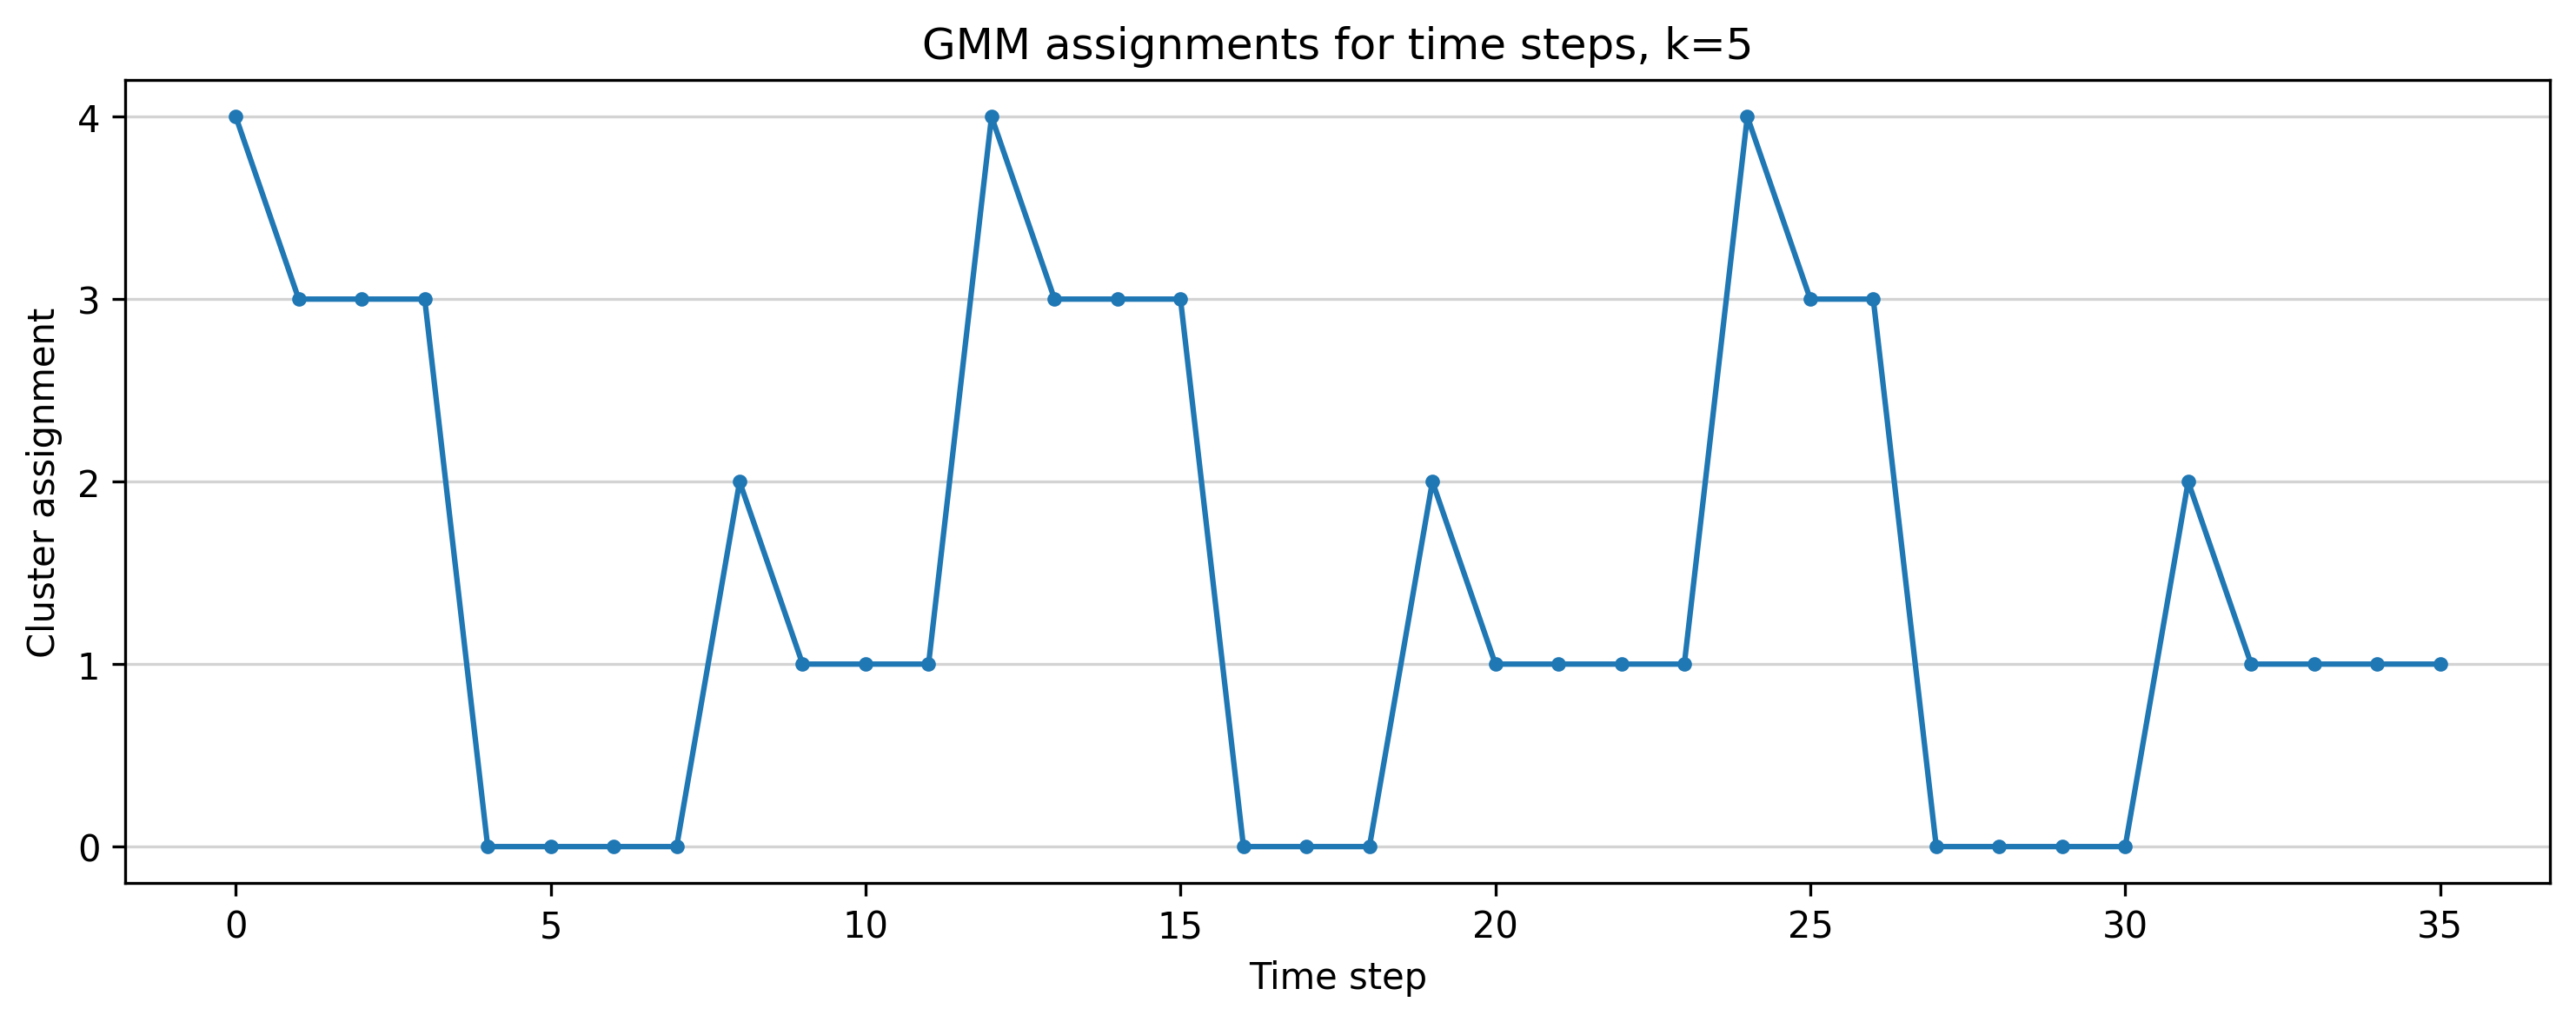
\includegraphics[scale=0.5]{figures/rough-gmm-classes.png}

    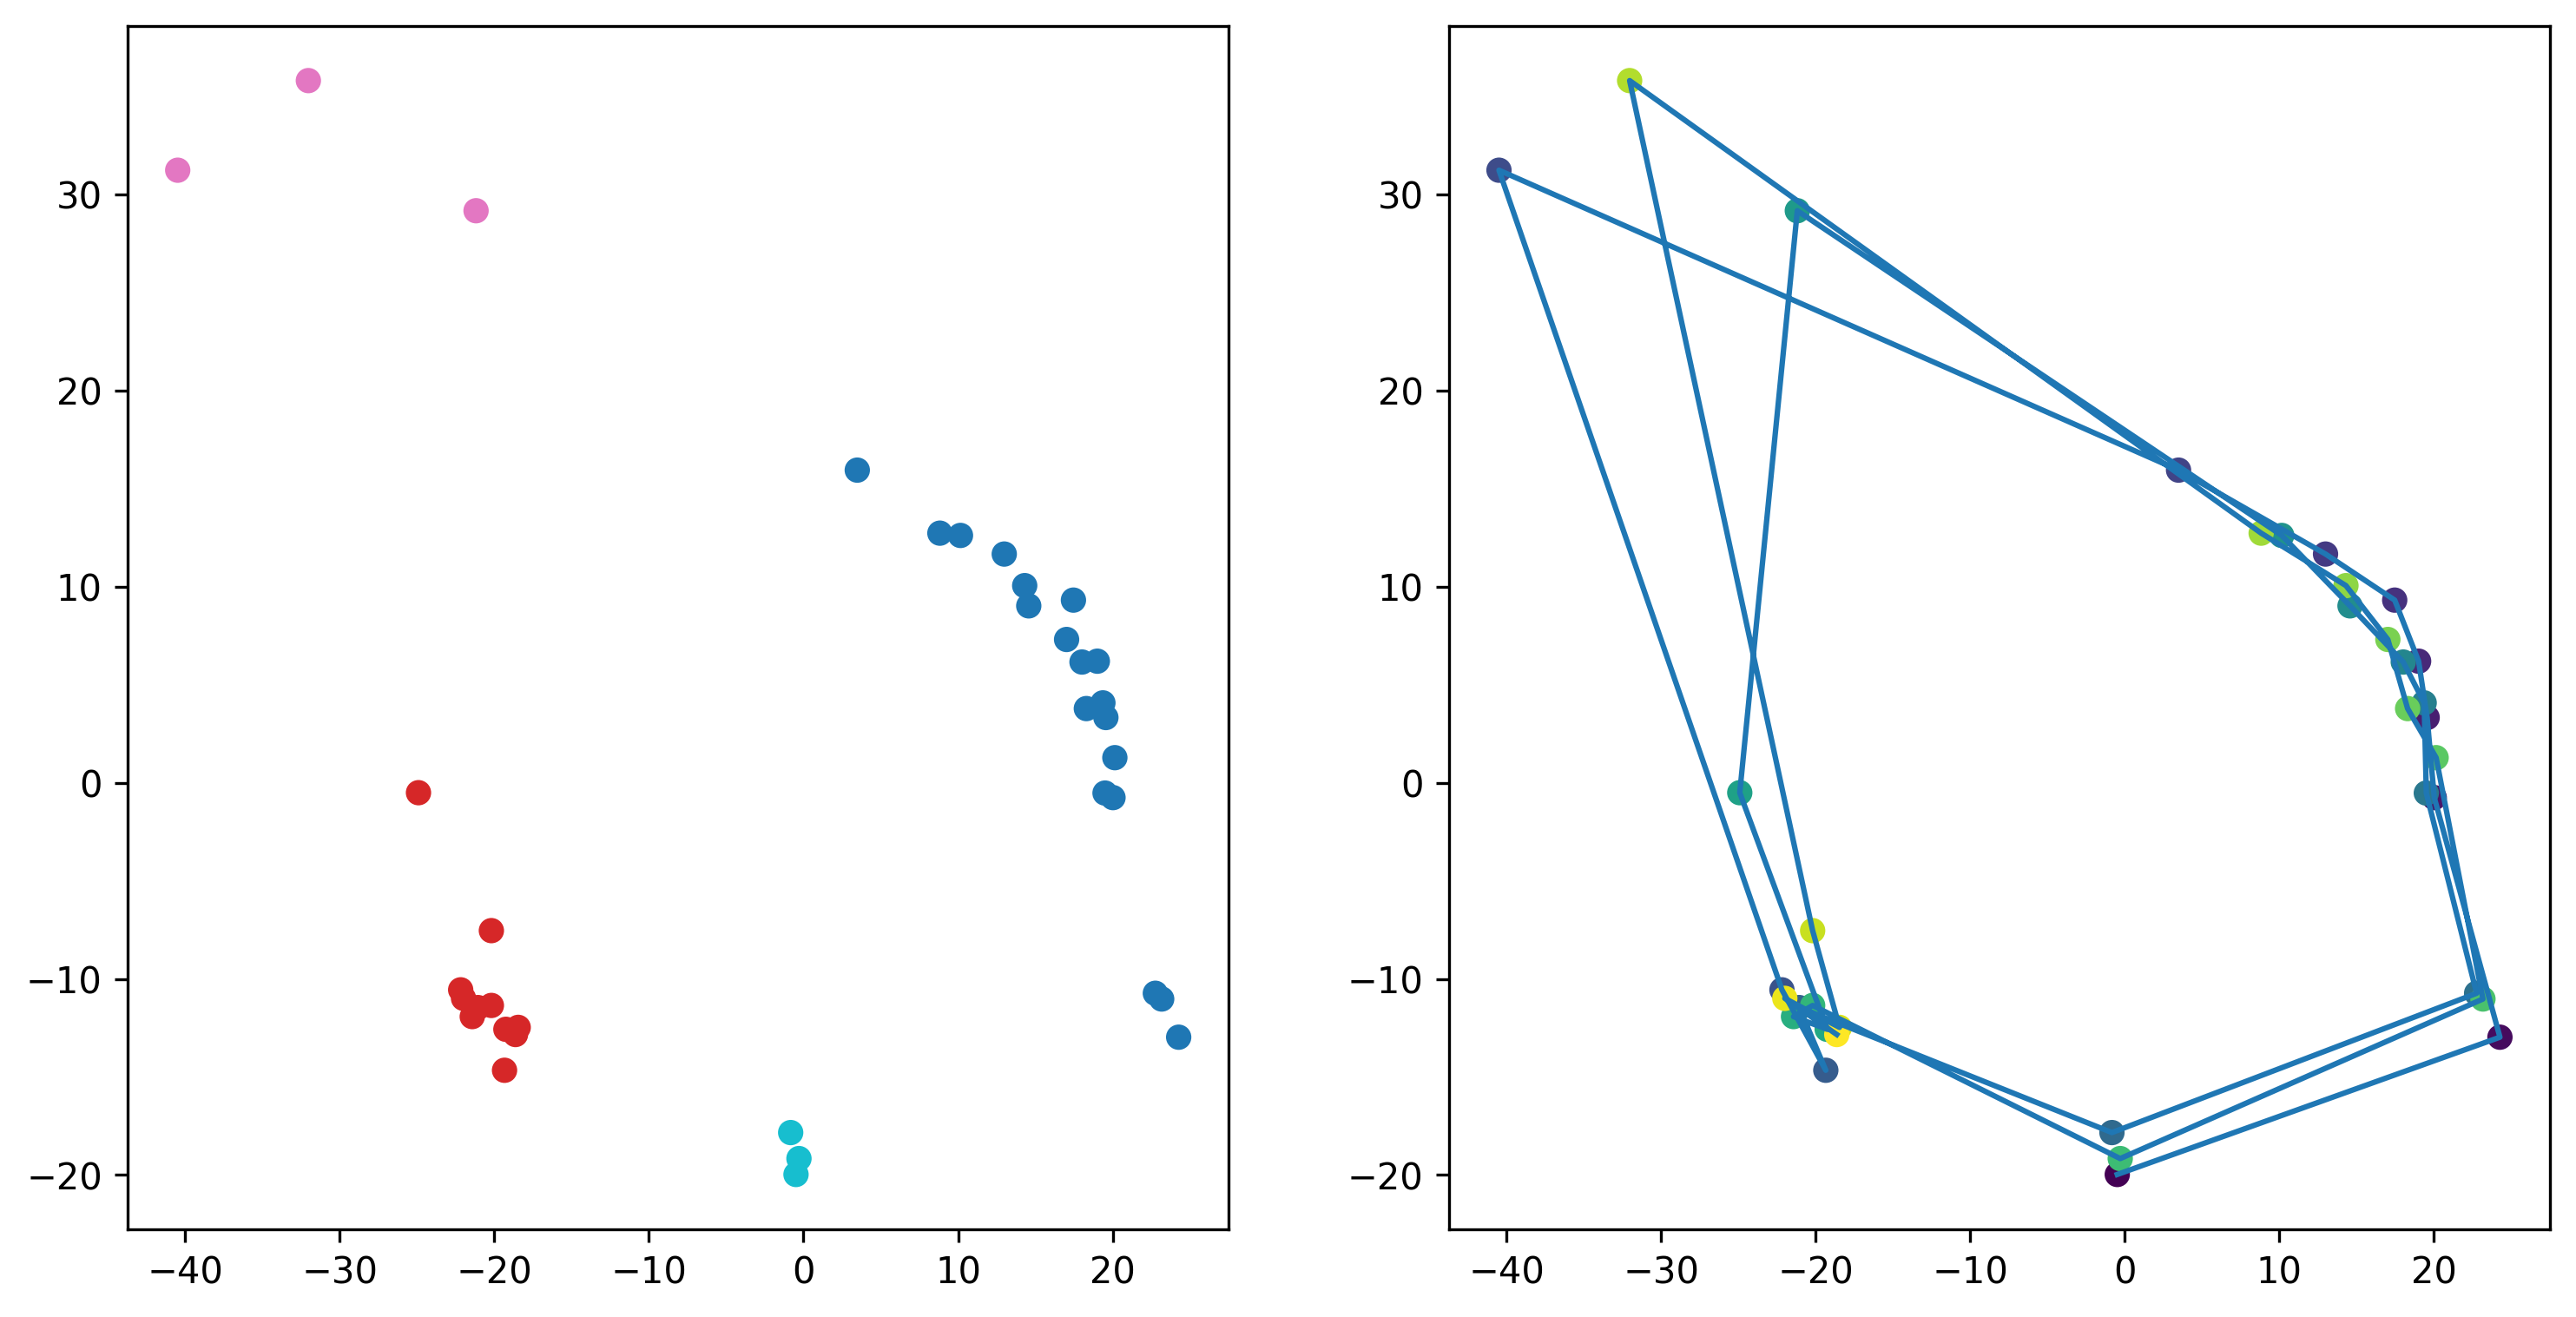
\includegraphics[scale=0.5]{figures/rough-cell-expression-cycles.png}

    \caption{A (top): GMM cluster assignments over time--the 12-time-step period is clear. B (bottom): Projection to two principal components of 200-dimensional time-steps, colored by GMM assignment and connected in order. The clusters and cycle are clear.}

    \label{fig:gmm}
\end{figure}

\textbf{Approach 3. Continuous Density Hidden Markov Model.} We also attempted to discover hidden states using a Continuous Density Hidden Markov Model (CDHMM) approach. We using PCA on our \textit{arcsin} normalized dataset to capture the directions of highest variance, and then used
\textit{GaussianHMM} method from the \textit{hiddenhmm} package on the transformed data to compute the hidden states. A CDHMM approach using 5 states shows robust periodicity (Figure \ref{fig:cdhmm}).

\begin{figure}[htbp]
    \centering
    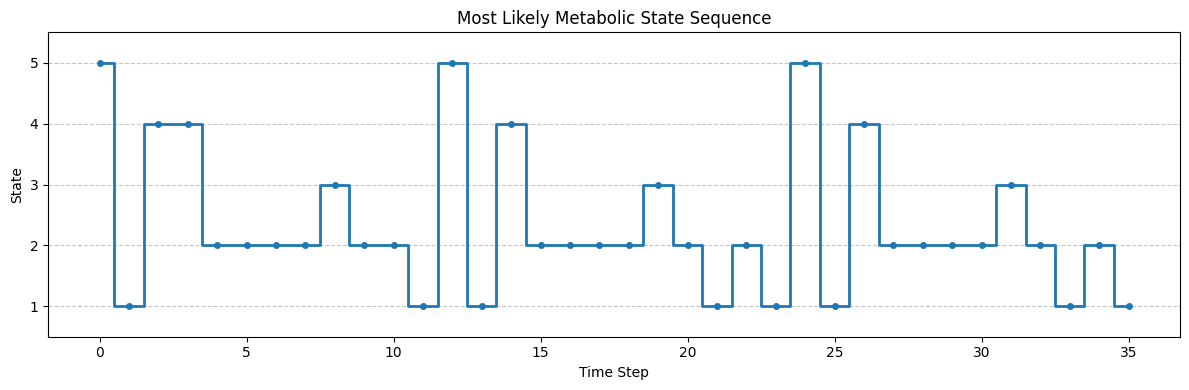
\includegraphics[width=0.99\textwidth]{figures/redone_metabolic_state.png}
    \caption{The hidden states predicted by a CDHMM approach over the course of the metabolic cycle also support an overall 12-timestep periodicity.}
    \label{fig:cdhmm}
\end{figure}

\subsection{Periodic Gene Identification}
Once an overall 12-timestep period length was identified, we used permutation testing to identify which of the 9725 transcripts were oscillatory on that period. We computed the autocorrelation of each transcript's time series with delay equal to the period length (12 timesteps). We called these values the \textit{true series autocorrelation} for each gene. We then randomized the order of the intensities in each time series 100 times and computed the lag-12 autocorrelations of these shuffled time series. If the absolute value of the true series autocorrelation was at the 95th percentile or greater relative to the absolute values of the randomized series, we accepted the gene as likely periodic and labeled it accordingly for downstream analyses. The other genes were rejected as non-periodic on the 12-timestep period, since significant numbers of randomized permutations of their time series had similar lag-12 autocorrelations.

We used PCA to visualize the distributions of expression patterns between the periodic and non-periodic genes. Our visualizations on the arcsinh-transformed relative intensities (Figure \ref{fig:periodicpca}A) appears consistent with the hypothesis that that both periodic and non-periodic genes can be found with wide ranges of average expression levels (appears consistent with PC1), while periodic genes otherwise vary more in the temporal modlulation of expression profiles than the non-periodic genes (appears consistent with PC2). To remove the variation in average expression between genes from the visualization, we also visualized the time-relativized (Z-scored) expressions with PCA (Figure \ref{fig:periodicpca}B), finding that in two dimensions, the time-relativized periodic time series tend to a wider distribution than the non-periodic genes, surrounding them with a disc or annulus-like shape.

\begin{figure}
    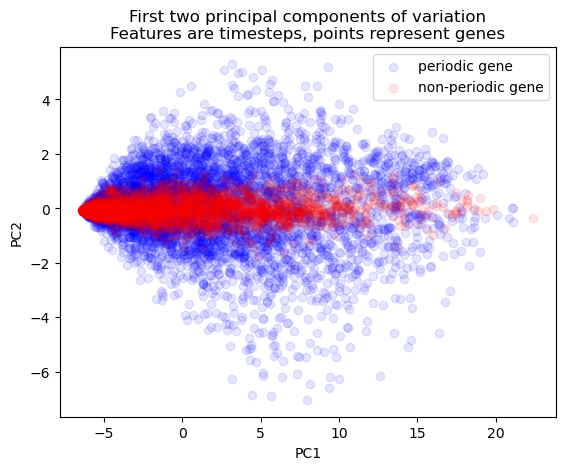
\includegraphics[scale=0.4]{figures/rough-periodic-gene.png}
    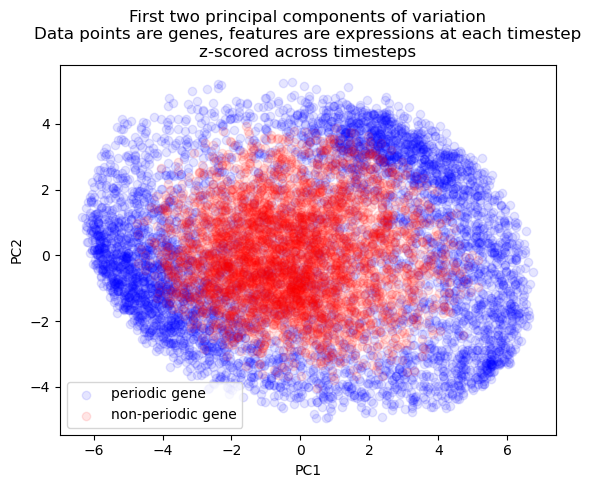
\includegraphics[scale=0.4]{figures/rough-periodic-normalized-gene.png}
    \caption{Distributional differences in the time series of periodic and non-periodic genes. A (left): A PCA plot of individual transcripts by their arcsinh-transformed relative intensities across timesteps. B (right): A similar plot, using the time-relativized (Z-scored) versions of those values.}

    \label{fig:periodicpca}
\end{figure}

\subsection{Classical Time Series Analysis}
Once a suitable overall period and individual periodic genes were identified, we used classical time series analysis to investigate the periodic genes specifically in more depth. We obtained the classical time series decomposition the arcsinh-transformed data for each individual gene via centered moving averages over the 24 central time steps (as the moving average requires timesteps at the beginning and end of the time series). We then Z-scored the seasonal components for each transcript across time points in that transcript's seasonal component. We clustered these Z-scored seasonal components used GMMs of varying cluster counts, finding 8 clusters to minimize the BIC values. We then inspected the individual transcript clusters in more depth through visualization.

Note that here we cluster \textit{transcripts}, whereas earlier we clustered \textit{time steps}. The time-step clustering recovered period-length, and the transcript clustering recovered distinct temporal modules of co-expressed transcripts.

\subsection{ARIMA}
We attempted to fit the data to an ARMA model. Largely, these efforts are unsuccessful. While we can fit individual genes as ARMA models, efforts to include interactions between genes failed. To try to combat the curse of dimensionality, we attempted to fit multivariate ARMA models to reduced data from PCA, or to the mean trends of clustered data. However, these attempts also failed, either due to lack of convergence or to nonsensical results. We attribute this result to the inherent periodicity in our data. This violates ARMA's assumption of a covariance stationary time series (the expected value of the time series is different at different time steps). In our case, first and second differencing (ARIMA) did not eliminate the problems, which makes sense because the trend was not linear or quadratic but oscillatory. Some literature search showed that seasonal differencing could be an appropriate solution for future work \cite{rob_j_hyndman_forecasting_2026}.

\subsection{Semantic Cluster Evaluation}
\textbf{TODO: Semantic Evaluation of Clusters via AI model}



%%Fourth Section
\section{Results and Analysis} 
% Clearly and succinctly describe your results. Give a thorough analysis and a thoughtful discussion of the conclusions that can be drawn.  Discuss the suitability and effectiveness of the different models and methods for the problems or questions treated.  
We first performed GMM clustering and fit a CDHMM across the time steps. The key takeaway was the recovery of the period of the yeast's metabolic cycle. Every method tried consistently recovered a 12 time-step period, or 300 minutes. Thus the dataset spans exactly three periods. The cluster assignments are near-deterministic, indicating well-separated phases. The high-dimensionality of the data and the relatively low number of timesteps makes this reasonable. For each iteration of GMM clustering and CDHMM fitting, $k=5$ hidden states was most robust, but the numer of clusters had no bearing on the recovered period of the metabolic cycle--all numbers of clusters recovered the same period with these methods.

The 300-minute period matches prior estimates of this particular metabolic process well, and our work independently verifies the period recovered by Tu et al.\ \cite{Tu2005}. We use knowledge of the period in downstream methods, such as for classical time series analysis, and the splitting of data into basically periodic and non-periodic. 



Armed with a knowledge of the period of the metabolic cycle, we can ask which genes oscillate, and when. We performed permutation testing to identify the genes with significant 12-timestep delay autocorrelations, in line with our conclusion that a 12 timestep period was most plausible. Via this analysis, 5243 of the genes - over half of all genes - were identified as periodic with the 12 timestep period. Dimensionality reduction via PCA and visualization showed a clear difference in the distributions of periodic and non-periodic genes.



After extracting the seasonal decomposition for each gene's time series using the mean- and variance-standardized data, we clustered these seasonal components, again using GMM clustering. We chose to use eight clusters, because this minimized the BIC and gave a local minima in the AIC.

Visualization of the seasonal components of normalized expression by cluster revealed distinct temporal modules of genetic expression in all but one cluster, with peaks or troughs of different shapes and sizes at different phases of the cycle. Of the 7 distinct clusters, visualization showed that two pairs of clusters appeared to be especially similar to one another, suggesting that perhaps a more natural cluster number would be 5 or 6. The remaining cluster appeared to represent a catchall for noisy time series that did not have a clear choice in cluster.

\textbf{TODO LDA results}

ARMA models were explored but failed to converge meaningfully due to the inherent nonlinearity of periodic data; see Methods §3.4.

\begin{figure}
    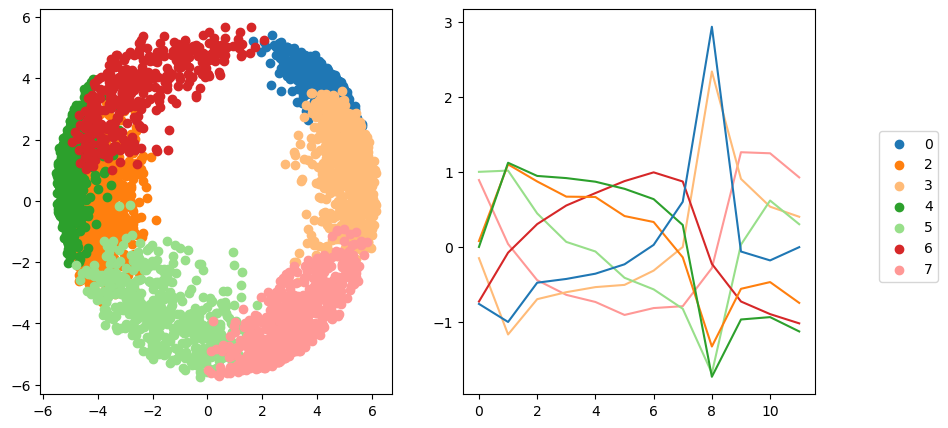
\includegraphics[scale=0.5]{figures/rough-seasonal-clusters.png}
    \caption{Temporal expression modules. [TODO: Cleanup + Label Graph] Left: UMAP of genes according to the seasonal component of their standardized periodic expressions, colored by GMM cluster. Right: The seven clearly consistent GMM clusters. The noisy cluster (1) was removed from the analysis.}
\end{figure}

%%Fifth Section
\section{Ethical Implications and Conclusions}
% Thoughtfully analyze the ethical implications of your research questions, the data you gathered, and the analysis that was performed.  Are there privacy or other implications from the collection or use of the data?  Could your results and methods be misused or misunderstood?  What can and should be done to prevent misuse and misunderstanding?  Could your algorithms and methods result in a destructive self-fulfilling feedback loop?  How could that be prevented or controlled?  What other ethical implications does your work have?  
Interpretation and analysis of large genomic or transcriptomic data sets is becoming a canonical use case for the application of various data analysis techniques like the ones used here. Using a strategy of analyzing data using various techniques and at various levels of data dimension reduction can provide novel insights into the dataset being studied, and when several techniques converge to the same conclusion, our results obtain an additional robustness. 
In an era when the biological sciences are becoming increasingly under strain by a crisis of reproducibility and replication, the ability to produce consistent conclusions when reexamining and validating the analysis of a dataset is critical. 

Obviously, mathematical evaluation of mathematical data does $\textit{not}$ address the crux of this crisis - replication, where an experiment is repeated to validate previous results. However, when replication is situationally challenging, developing robust strategies of reproducibility can strengthen the credibility of scientific researchers and strengthen their conclusions. Thus, deployment of various strategies to analyze complicated, high-dimensional data is important both to gain novel insights into experimental data, but also to validate previous conclusions about a dataset. Prudent, robust, and comprehnsive
approaches to reproducibility lends additional credibility to experimental conclusions, and thus is a boon to the credibility of modern biological sciences as a whole.



%% Sixth section
\section{Conclusion} 
% Describe the final conclusions that you draw from your computations, results, and analysis. 
Analyzing the data provided an independent confirmation of some of the conclusions of Tu et al.\ \cite{Tu2005}. For example, the period they identified from the data (300 minutes) for the yeast metabolic cycle oscillations via a maximum likelihood analysis was rediscovered by our independent use of GMMs to cluster the timesteps, and we likewise identified slightly more than half of the dataset's genes as periodic with this period. This concordance reinforces the strength of those conclusions about their data. We also were able to provide novel analyses and interpretations of the data that Tu et al.\ did not reach. For example, our extraction of the seasonal components of the standardized time series and our use of GMMs to cluster them revealed 5-7 distinct periodic modules of activation, which improves upon the granularity of the original analysis \cite{Tu2005}, which identified only three clusters using k-means. This increased granularity could lead to improved biological insight. 


%All text before this line should end before page 11 starts.
%%%%%%%%%%%%%%%%%%%%%%%%%%%%%%%%%%%%%
%% Bibliography below
%%%%%%%%%%%%%%%%%%%%%%%%%%%%%%%%%%%%%
\FloatBarrier % Keep all figures from being put after the bibliography
\newpage
%% If using bibtex, leave this uncommented
\bibliography{refs} %if using bibtex, call your bibtex file refs.bib
\bibliographystyle{alpha}

%% If not using bibtex, comment out the previous two lines and uncomment those below
%\begin{thebibliography}{99}
%\bibitem{Vandermeersch} First reference goes here
%\end{thebibliography}

\end{document}
